\chapter{Materiales y Métodos}
\section{Materiales}
\subsection{Conjunto de datos genéricos} 
\label{sec:DatosPublicos}
Para este TFG se han utilizado diversos conjuntos de datos públicos para la 
evaluación y elección de los modelos anteriormente descritos. De entre ellos 
están SJTU~\cite{SJTU}, WPC~\cite{WPC1,WPC2} y LS-PCQA~\cite{ResSCNN} que tratan 
de conjuntos de nubes de puntos generalistas, de personas, animales y objetos.

El primero de ellos parte de 10 nubes de puntos de referencia (véase Figura \ref{fig:SJTU}), 
a las cuales se aplican 7 tipos de distorsiones. Estas son: compresión, ruido 
al color, ruido geométrico, ruido gaussiano y combinación entre ellas (véase Tabla \ref{tab:SJTU}). Todas se aplican en una escala creciente
de intensidad del 1 al 6. Luego, se obtiene un MOS de 10 individuos para las 420 
nubes de puntos que sirve como medida de calidad de las mismas y para evaluar las predicciones del modelo.

\begin{figure}[htp]
  \centering 
    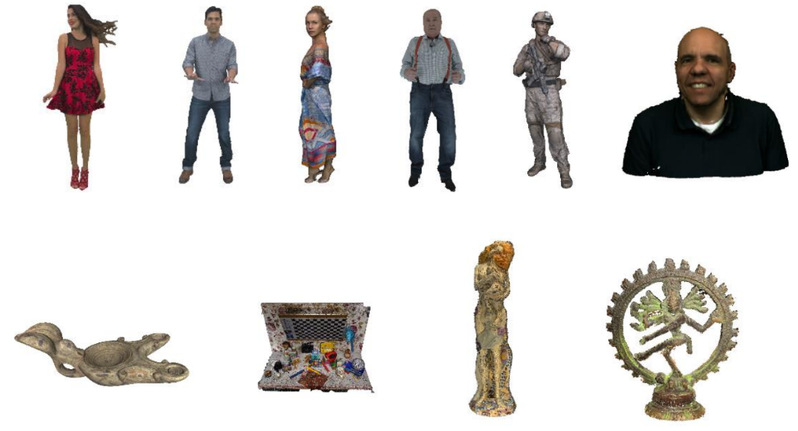
\includegraphics[width=0.75\textwidth]{imagenes/chapter4/SJTU}
    \caption{Ejemplo de conjuntos de datos SJTU.}
    \label{fig:SJTU}
\end{figure}

\begin{table}[htp]
  \centering 
  \scriptsize
  \begin{tabular}{|c|c|}
    \hline
    \rowcolor[HTML]{FFC702}
    \textbf{Número} & \textbf{Tipo de Distorsión} \\ 
    \hline 
    0 & OT: Compresión octree~\cite{OctreeCompression} \\ 
    \hline 
    1 & CN: Ruido fotométrico\\ 
    \hline 
    2 & DS: Submuestreo uniforme \\
    \hline 
    3 & DS + CN \\
    \hline 
    4 & DS + GGN \\
    \hline 
    5 & GGN: Ruido geométrico gaussiano \\
    \hline 
    6 & CN + GGN \\ 
    \hline 
  \end{tabular}
  \caption{Ejemplo de distorsiones en SJTU.}
  \label{tab:SJTU}
\end{table}

El segundo dataset, WPC~\cite{WPC1, WPC2}, también posee distorsiones como submuestreo uniforme y 
ruido gaussiano (aplicados de manera distinta), pero a su vez posee nuevos tipos 
de distorsiones. Estos son basados en distintos tipos de compresión: V-PCC, G-PCC y \emph{trisoup}.
Además, posee distintos tipos de nubes de puntos (véase Figura \ref{fig:WPC}) que 
pueden influir en el rendimiento del modelo si el conjunto no es
suficientemente amplio y representativo de lo que puede encontrarse una vez entrenado. 

\begin{figure}[htp]
  \begin{center}
    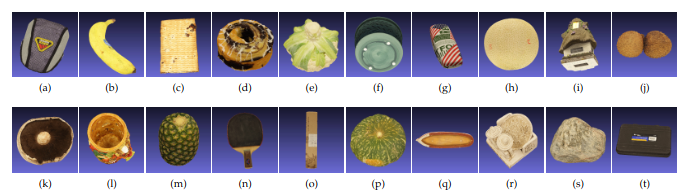
\includegraphics[width=0.95\textwidth]{imagenes/chapter4/WPC}
  \end{center}
  \caption{Ejemplo de conjunto de datos WPC.}
  \label{fig:WPC}
\end{figure}

Los dos anteriores han sido utilizados sobre todo para la evaluación y elección 
del modelo de regresión a utilizar. Son los conjuntos de datos más conocidos 
y que habitualmente están presentes en las publicaciones más recientes. Además, se realizaron 
pruebas de ejecuciones de algunos métodos de código abierto para verificar los 
resultados. Sin embargo, es el último el que finalmente se utiliza para entrenar un modelo para estimar 
la calidad de las imágenes médicas. Esto es porque LS-PCQA~\cite{ResSCNN} 
es el mayor conjunto de datos, en el momento de escritura, y posee tipos de distorsiones que pueden simular 
lo que sería ciertos errores y ruidos presentes en imágenes médicas. Por ejemplo, 
el ruido gaussiano (simular errores de transmisión y almacenado de datos), 
rotación y movimiento local (simular el movimiento del paciente) y compresión 
octree y por submuestreo uniforme (algoritmos de compresión comúnmente usados).
Aparte, es el con mayor amplitud de modelos base, con distintos tipos y categorías 
de objetos (véase Figura \ref{fig:LS-PCQA}).

\begin{figure}[htp]
  \begin{center}
    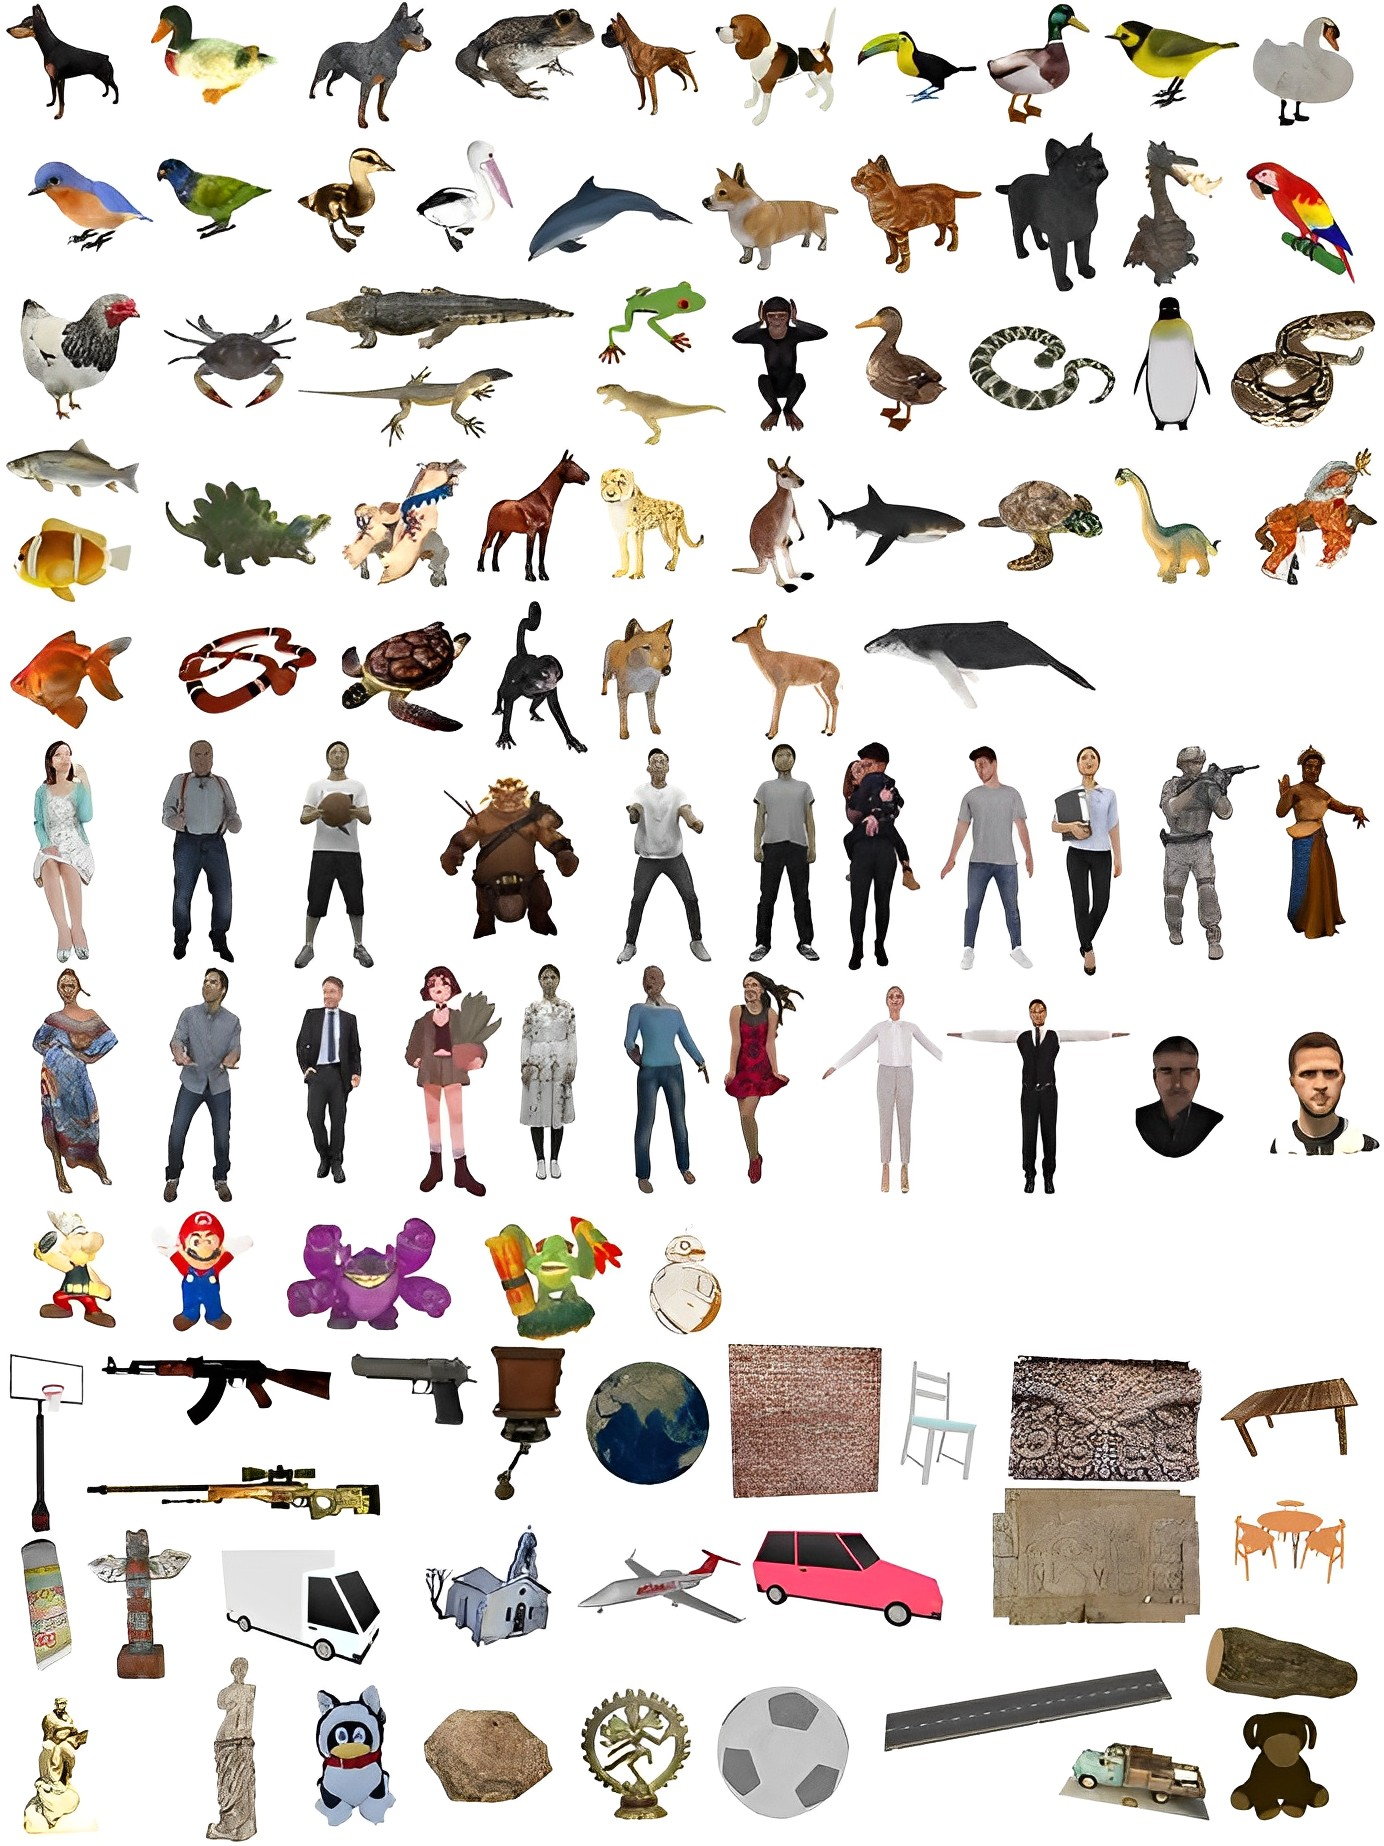
\includegraphics[width=\textwidth]{imagenes/chapter4/LSPCQA}
  \end{center}
  \caption{Ejemplo de conjunto de datos LS-PCQA.
  Vemos que en este conjunto de datos tenemos una gran variedad de nubes 
de puntos. 
En las primeras filas tenemos un conjunto de modelos de animales, 
seguidos de representaciones de seres humanos y, por último, 
varios objetos abstractos.}
  \label{fig:LS-PCQA}
\end{figure}

\subsection{Conjunto de datos médicos}
\label{sec:OurData}
Para este TFG se tiene disponible una conjunto de tomografías computarizadas, de diferentes
partes del cuerpo, de 2 individuos distintos del conjunto de datos públicos NMID~\cite{NMID}. 
De los cuales han sido segmentados las clavículas, el seno frontal y los senos maxilares. 
A parte, disponemos de modelos generados mediante escáner láser 3D, en concreto con el dispositivo Artec Spider, que permite generar reconstrucciones 3D de objetos reales. Estos modelos 3D fueron adquiridos en el Departamento de Medicina Legal, Toxicología y Antropología Física de la Universidad de Granada y constan del cráneo de otros 3 individuos, una pubis izquierda y
una pubis derecha (véase Figura \ref{fig:OurDataExample}). Es decir, en total disponemos de 11 nubes de puntos de alta 
calidad, que representan distintos volúmenes de exámenes médicos.
A estos datos no se hicieron ningún tipo de pre-procesado, apenas se centraron 
las nubes de puntos a los ejes (operación necesaria para hacer la rotación para 
las distintas perspectivas, más detalles en el Apéndice \ref{sec:Implementacion})
y se eliminaron aquellos puntos aislado de todos, frutos de errores en el 
algoritmo de reconstrucción 3D de las nubes de puntos a partir de segmentaciones DICOM. 

\begin{figure}[htp]
  \centering
  \begin{subfigure}[b]{0.40\textwidth}
  \centering 
  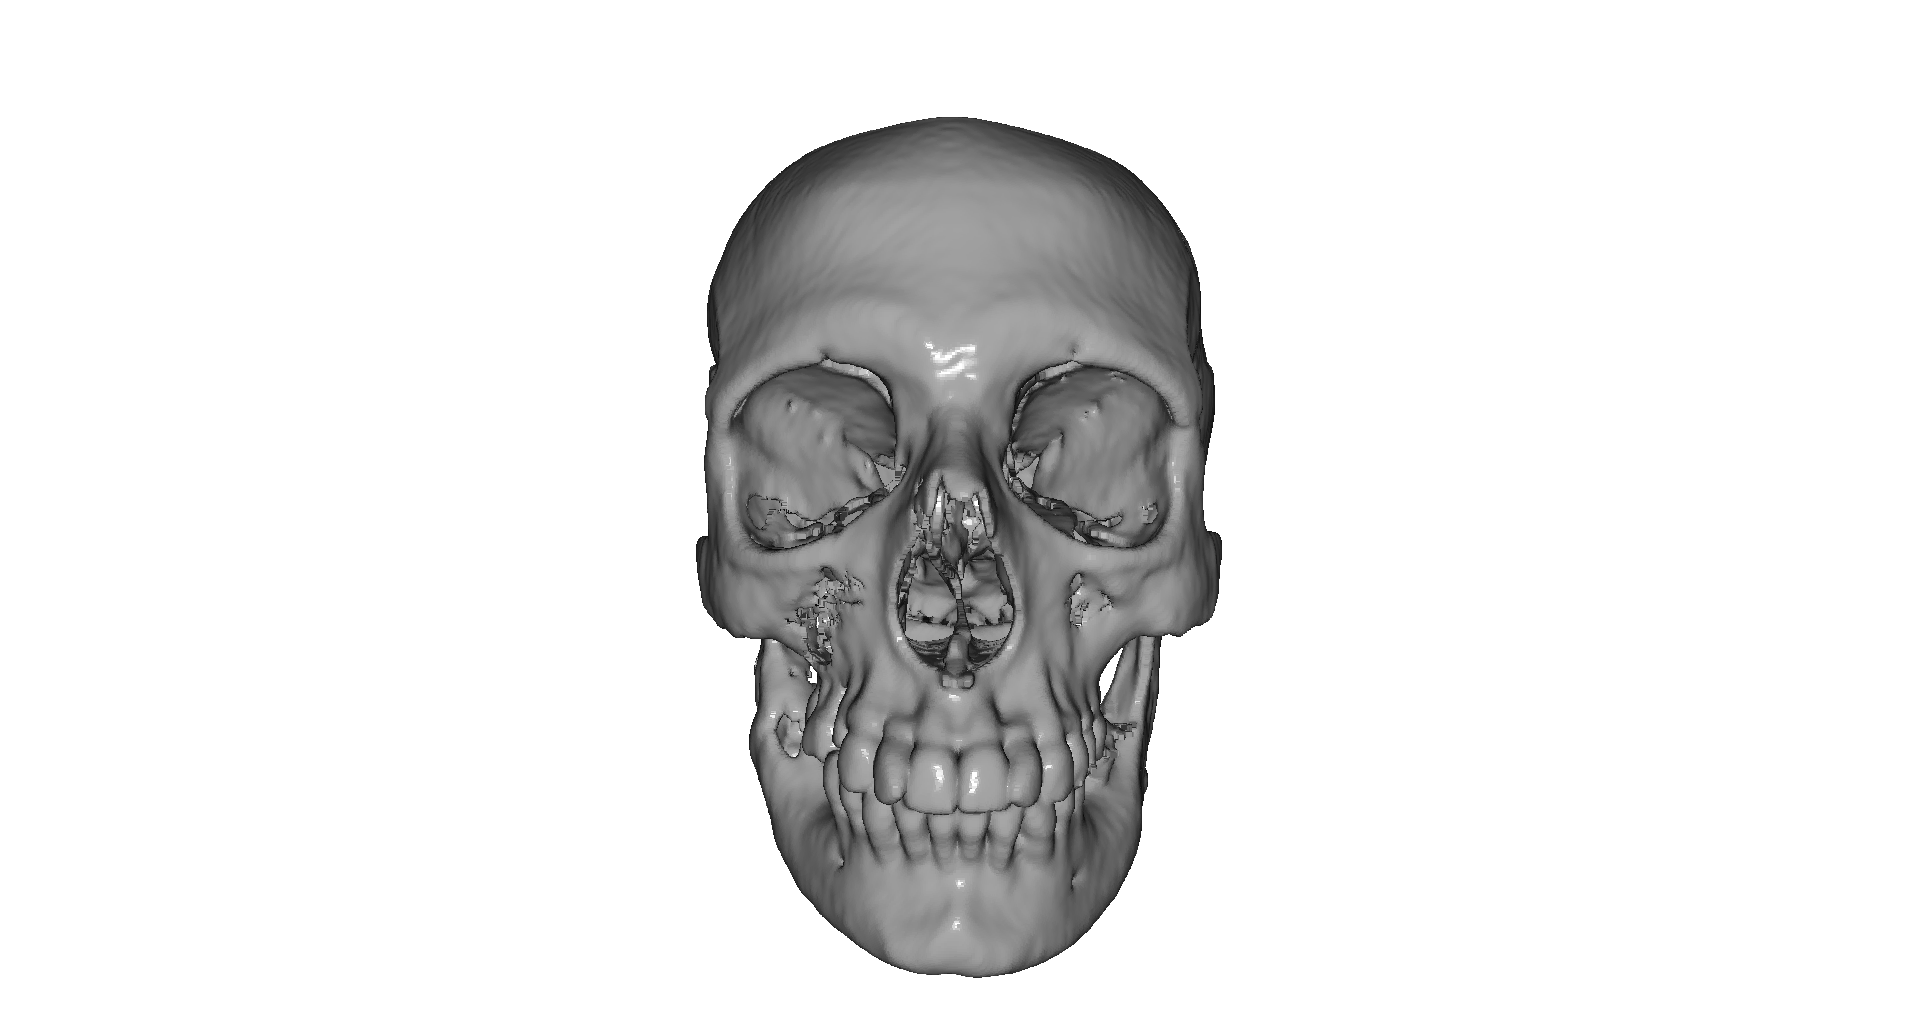
\includegraphics[width=\textwidth]{imagenes/chapter4/Craneo12018377.png}
  \end{subfigure}
  \begin{subfigure}[b]{0.40\textwidth}
  \centering 
  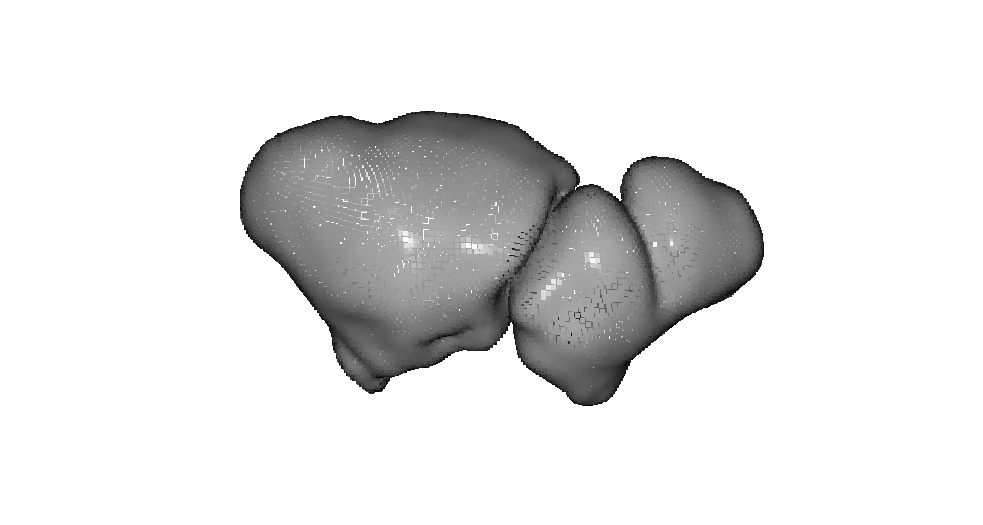
\includegraphics[width=\textwidth]{imagenes/chapter4/SenoFrontal100205.png}
  \end{subfigure}

  \begin{subfigure}[b]{0.40\textwidth}
  \centering 
  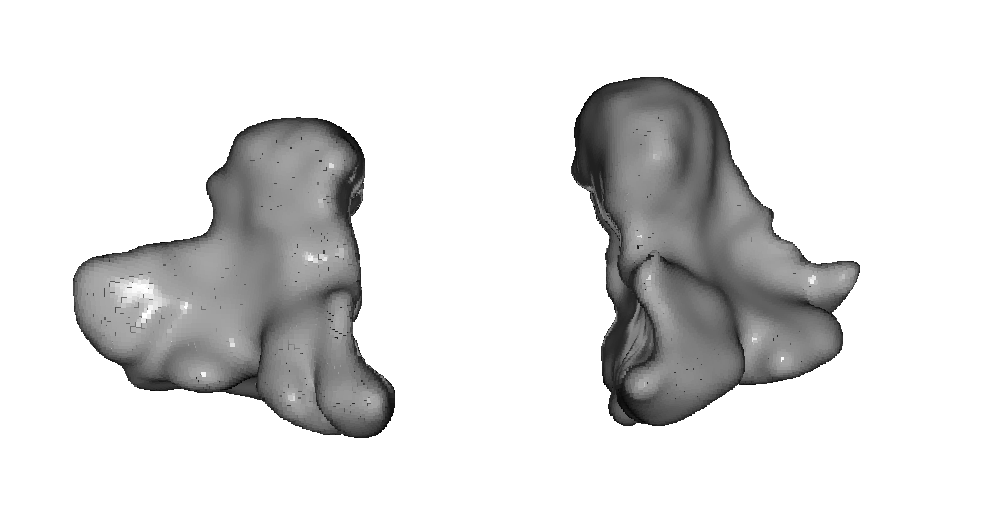
\includegraphics[width=\textwidth]{imagenes/chapter4/Maxilar100205.png}
  \end{subfigure}
  \begin{subfigure}[b]{0.40\textwidth}
  \centering 
  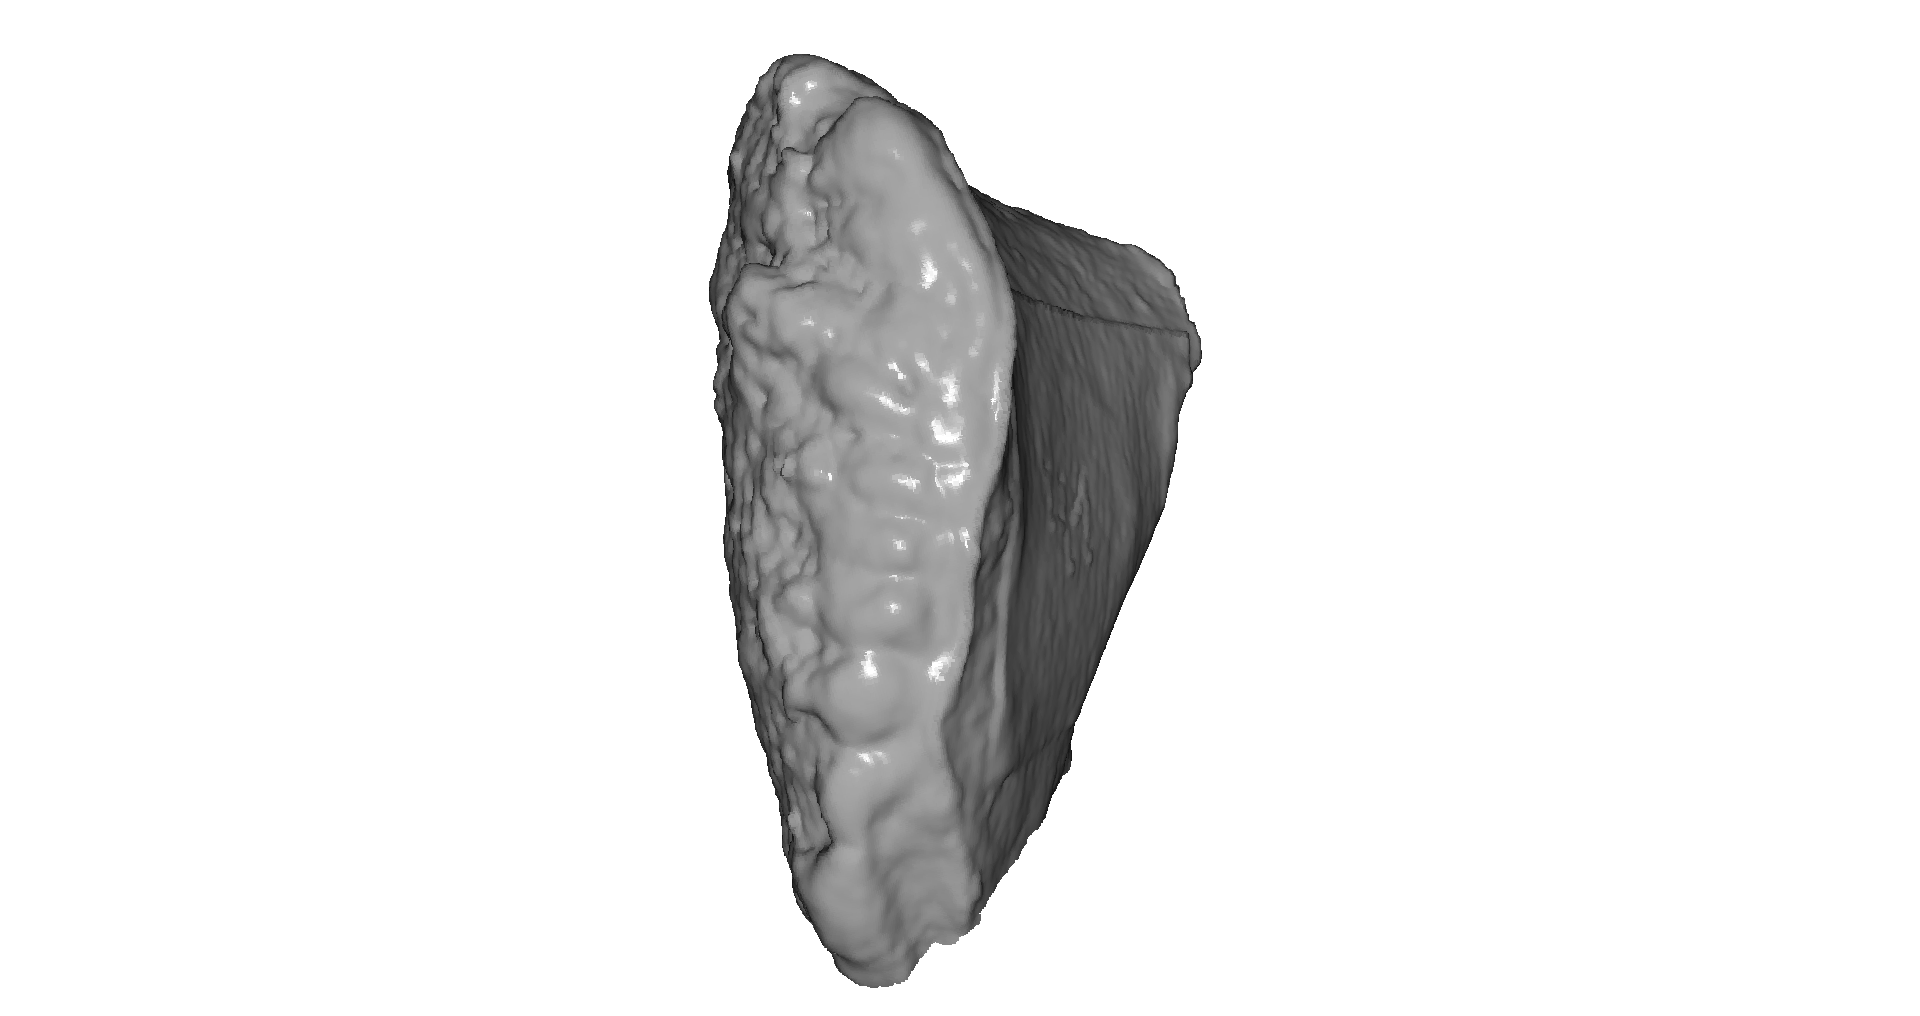
\includegraphics[width=\textwidth]{imagenes/chapter4/PubisDch.png}
  \end{subfigure}
  \caption[Ejemplo de nuestras imágenes médicas.]{Ejemplo de nuestras imágenes médicas.
  Arriba a la izquierda tenemos un cráneo y a su derecha un seno frontal. 
  Abajo a la izquierda tenemos un maxilar y a su derecha el pubis derecho.}
  \label{fig:OurDataExample}
\end{figure}


Cada nube de punto es centrada sobre los ejes como paso previo. A continuación, 
reducimos el número de puntos anormales analizando estadísticamente el vecindario de cada punto. 
A cada uno de estos ejemplos disponibles, se les aplica las 5 distorsiones médicas
discutidas en la Sección \ref{sec:Distorsiones}. 
Para simular dichas distorsiones, partiremos de todos los ejemplos de imágenes médicas 
mencionados anteriomente, considerados exentos de desperfectos. Dichos ejemplos 
están segmentados por profesionales. 

Dos de las distorsiones serán para simular los resultados de varios algoritmos de 
compresión, como puede ser \emph{octree compression}~\cite{OctreeCompression} 
y la reducción de número de puntos por medio de submuestreo aleatorio (en inglés \emph{random downsampling}). 
Un \emph{octree} es una representación más eficiente que los vóxeles, se trata 
de la descomposición de forma recursiva de la escena en 8 partes hasta 
la profundidad máxima, donde cada nodo representa un cubo tridimensional 
llamado octante. En la compresión se analiza los octantes y se elimina los que aportan 
menos información. 
En el segundo, establecemos un porcentaje de puntos que eliminar y los eliminamos 
de forma aleatoria hasta alcanzar ese porcentaje de reducción.
Las demás representarán efectos que podrían ocurrir por desplazamiento de los puntos, 
como el movimiento del paciente y aquellos provocados por ruido en la transmisión de datos.

\begin{figure}[htp]
  \begin{subfigure}[b]{.5\textwidth}
    \centering
    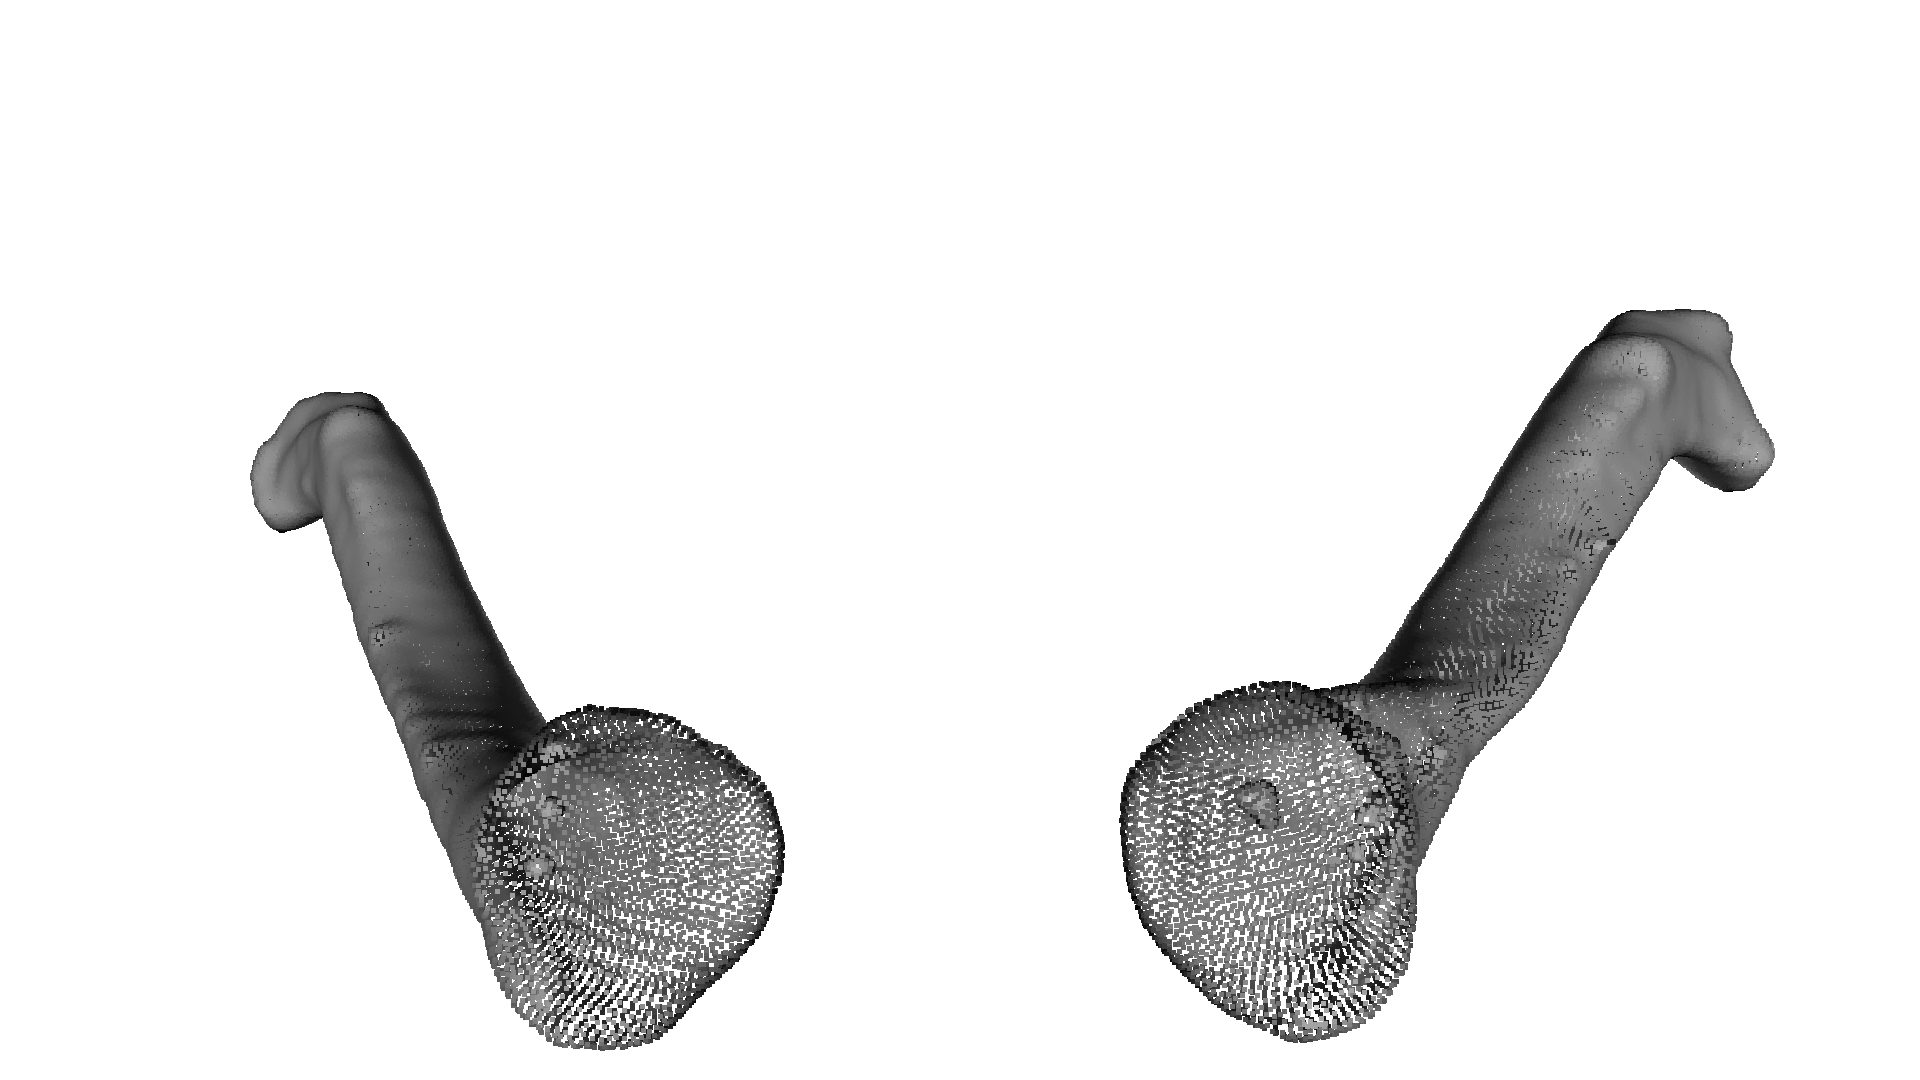
\includegraphics[width=.95\textwidth]{imagenes/chapter2/clavicula/clavicula_0.png}
    \caption{}
  \end{subfigure}
  \hfill
  \begin{subfigure}[b]{.5\textwidth}
    \centering
    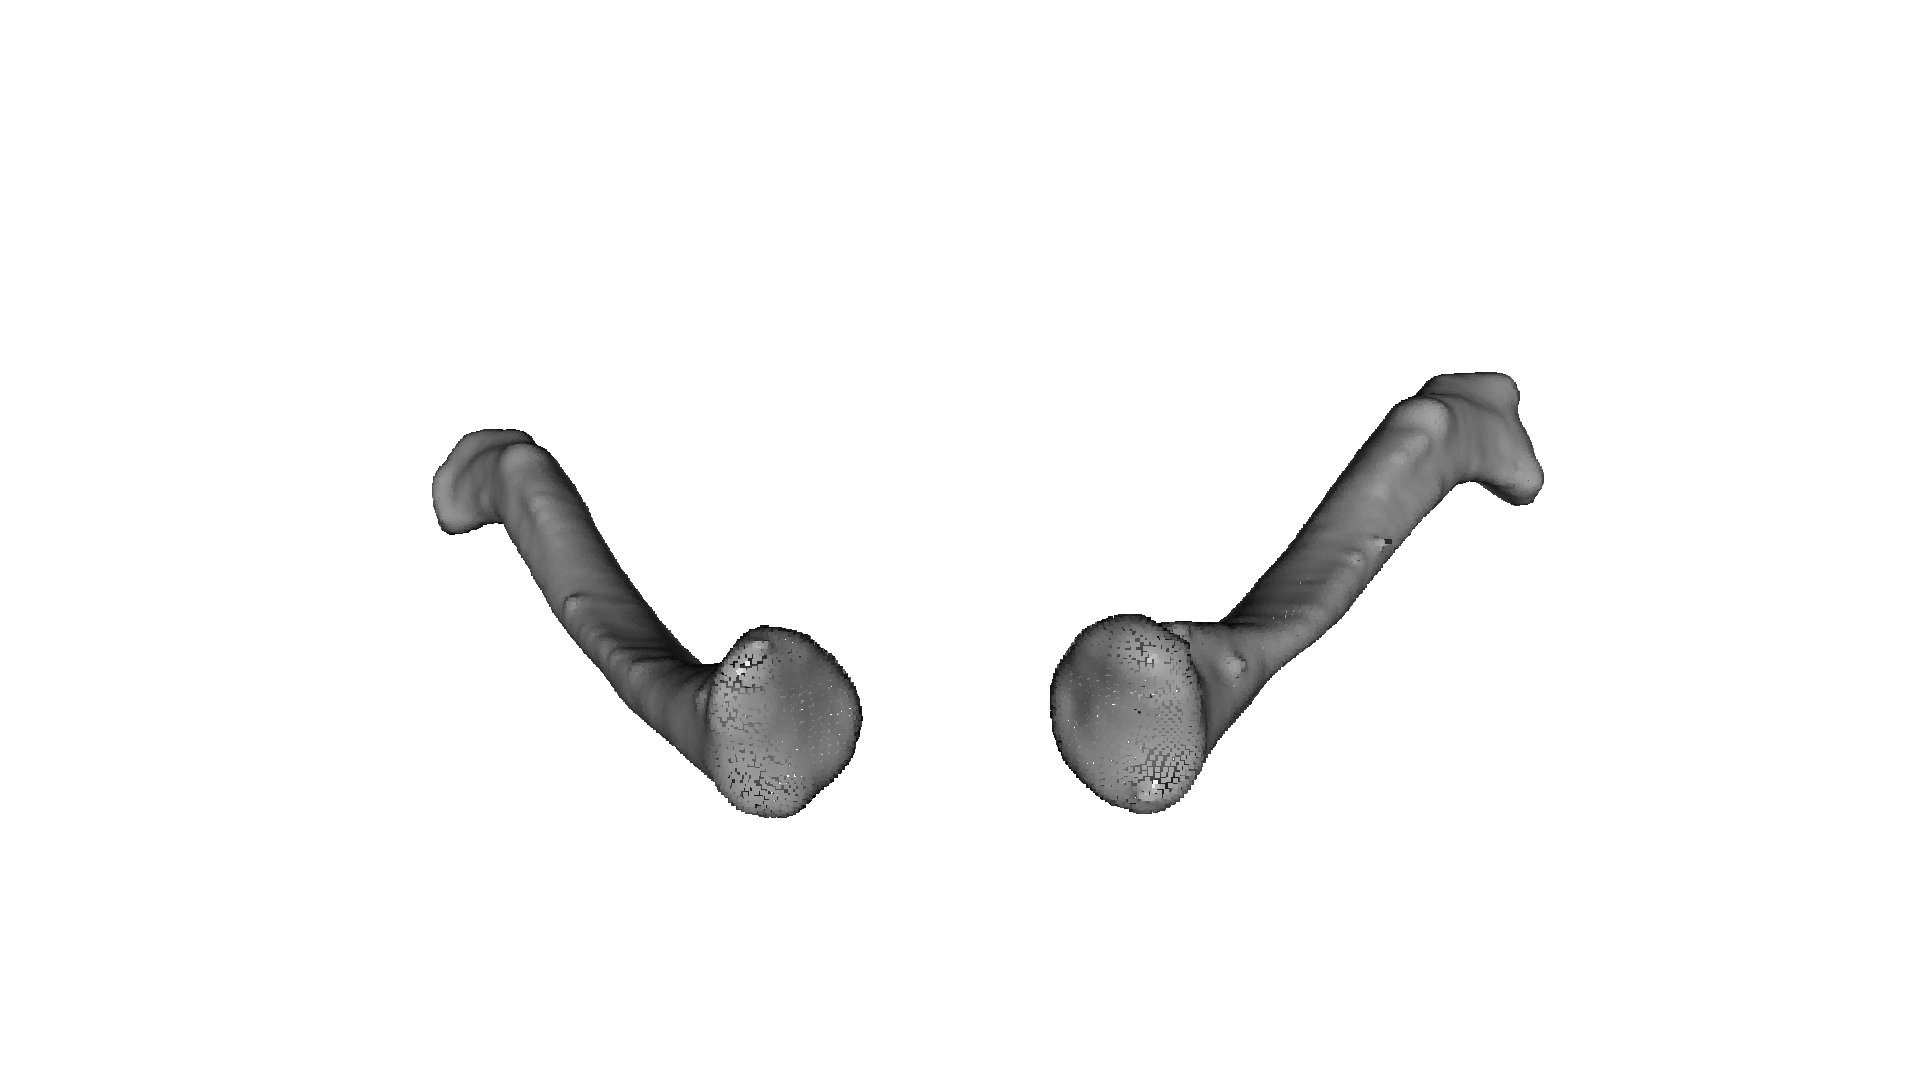
\includegraphics[width=.95\textwidth]{imagenes/chapter2/clavicula/clavicula_1.png}
    \caption{}
  \end{subfigure}
  \begin{subfigure}[b]{.5\textwidth}
    \centering
    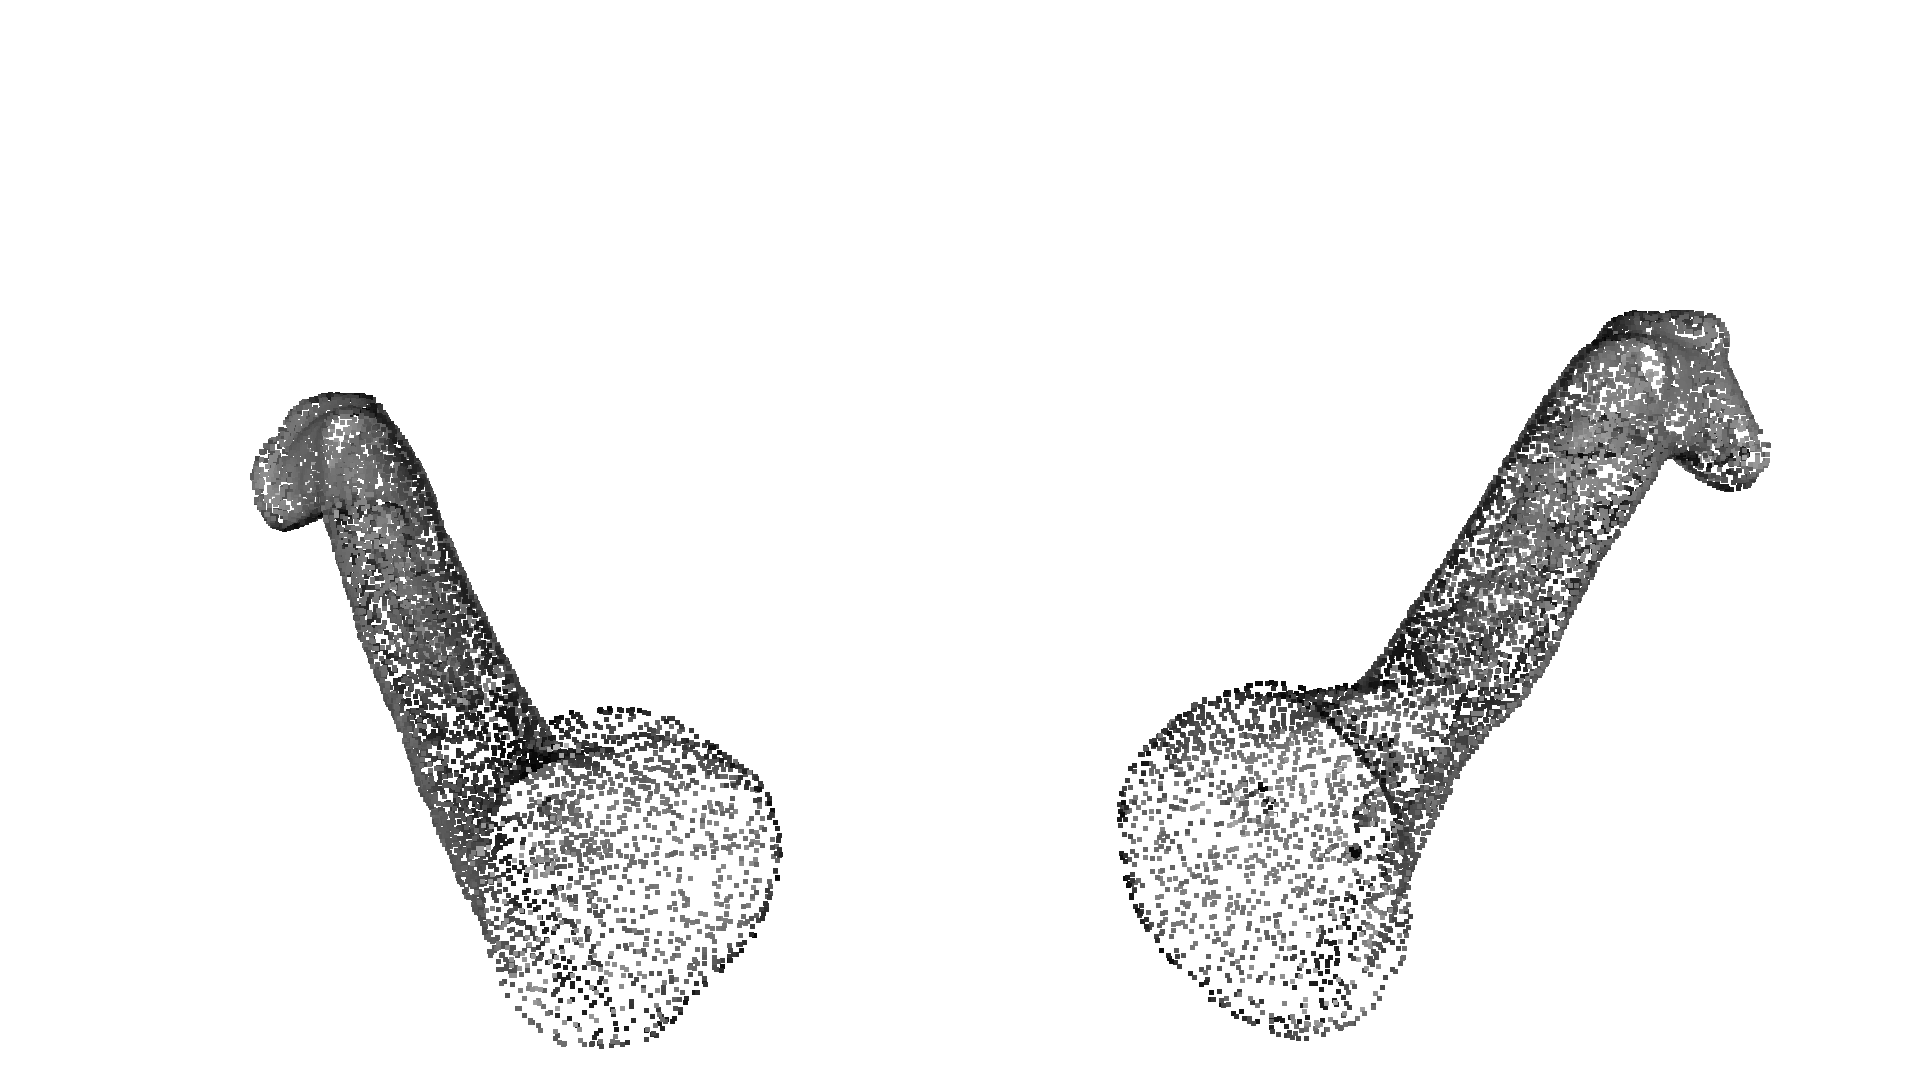
\includegraphics[width=.95\textwidth]{imagenes/chapter2/clavicula/clavicula_2.png}
    \caption{}
  \end{subfigure}
  \hfill
  \begin{subfigure}[b]{.5\textwidth}
    \centering
    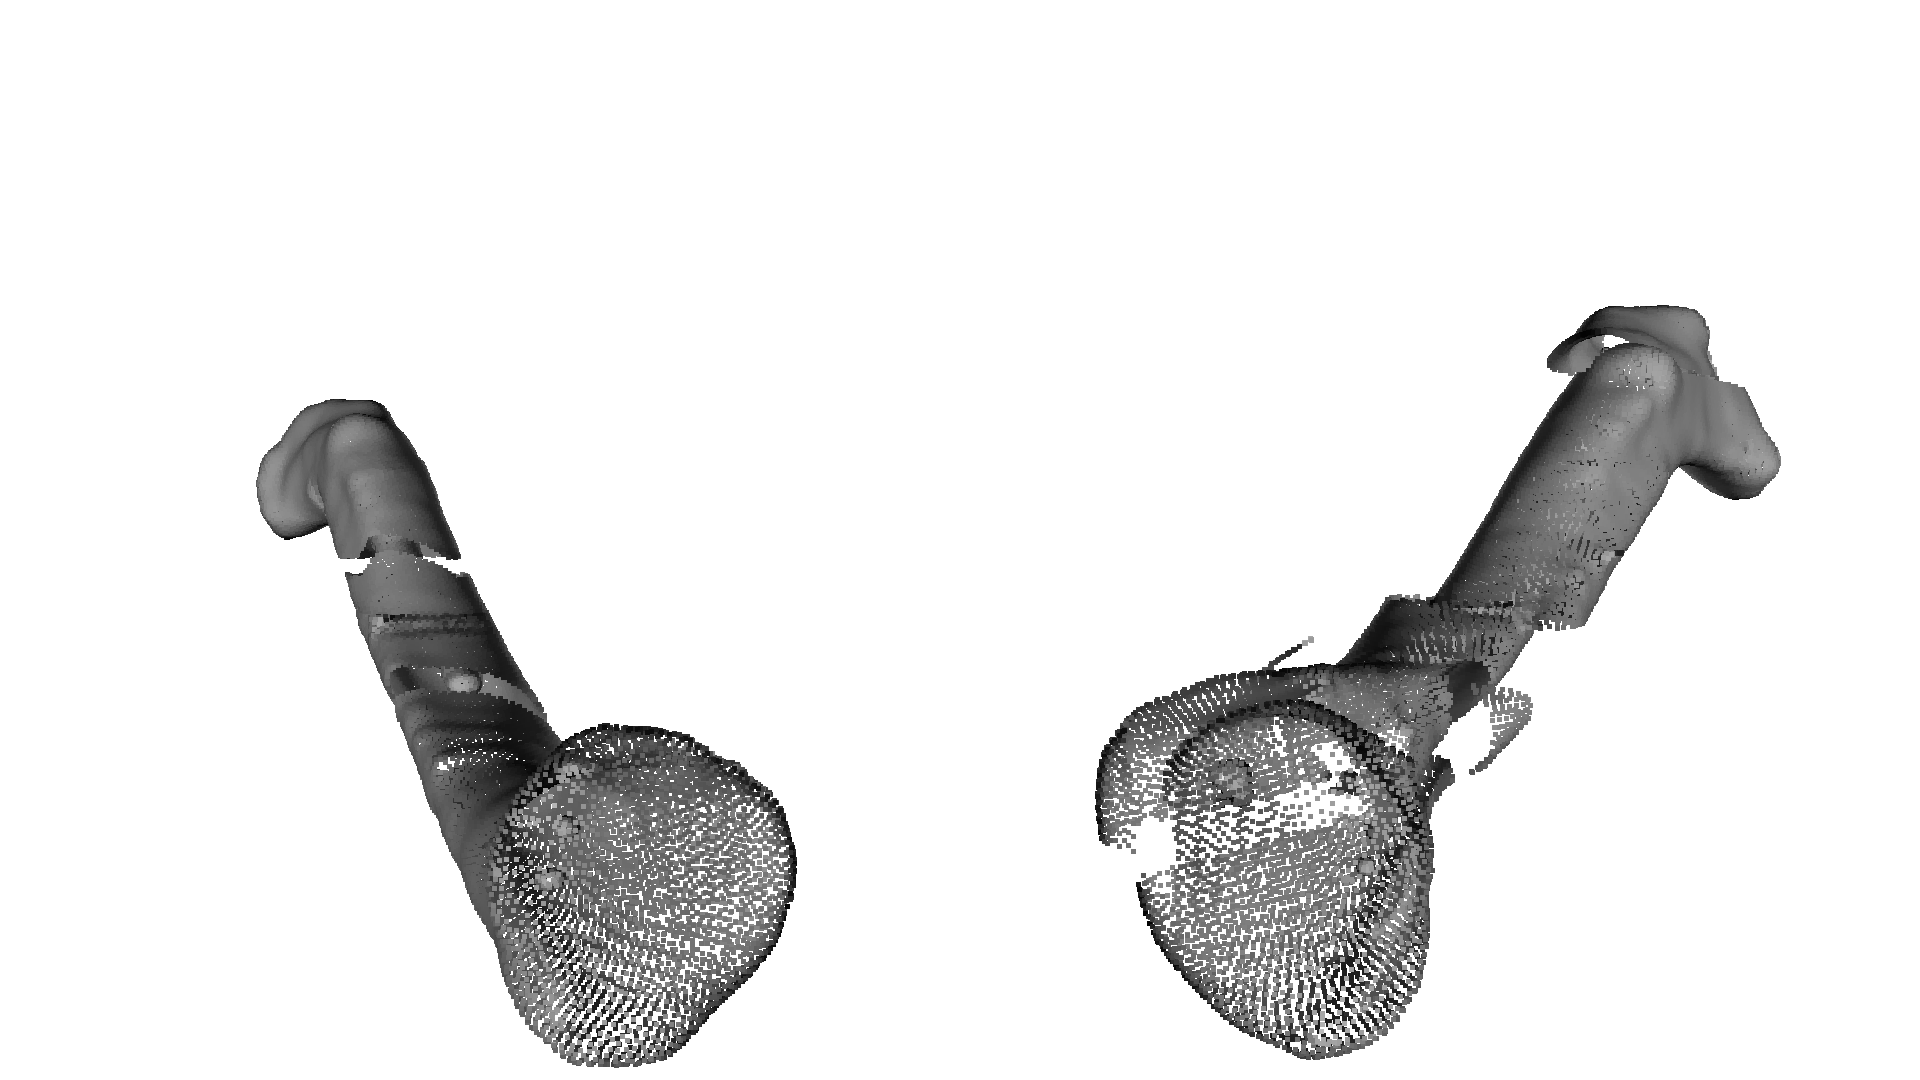
\includegraphics[width=.95\textwidth]{imagenes/chapter2/clavicula/clavicula_3.png}
    \caption{}
  \end{subfigure}
  \begin{subfigure}[b]{.5\textwidth}
    \centering
    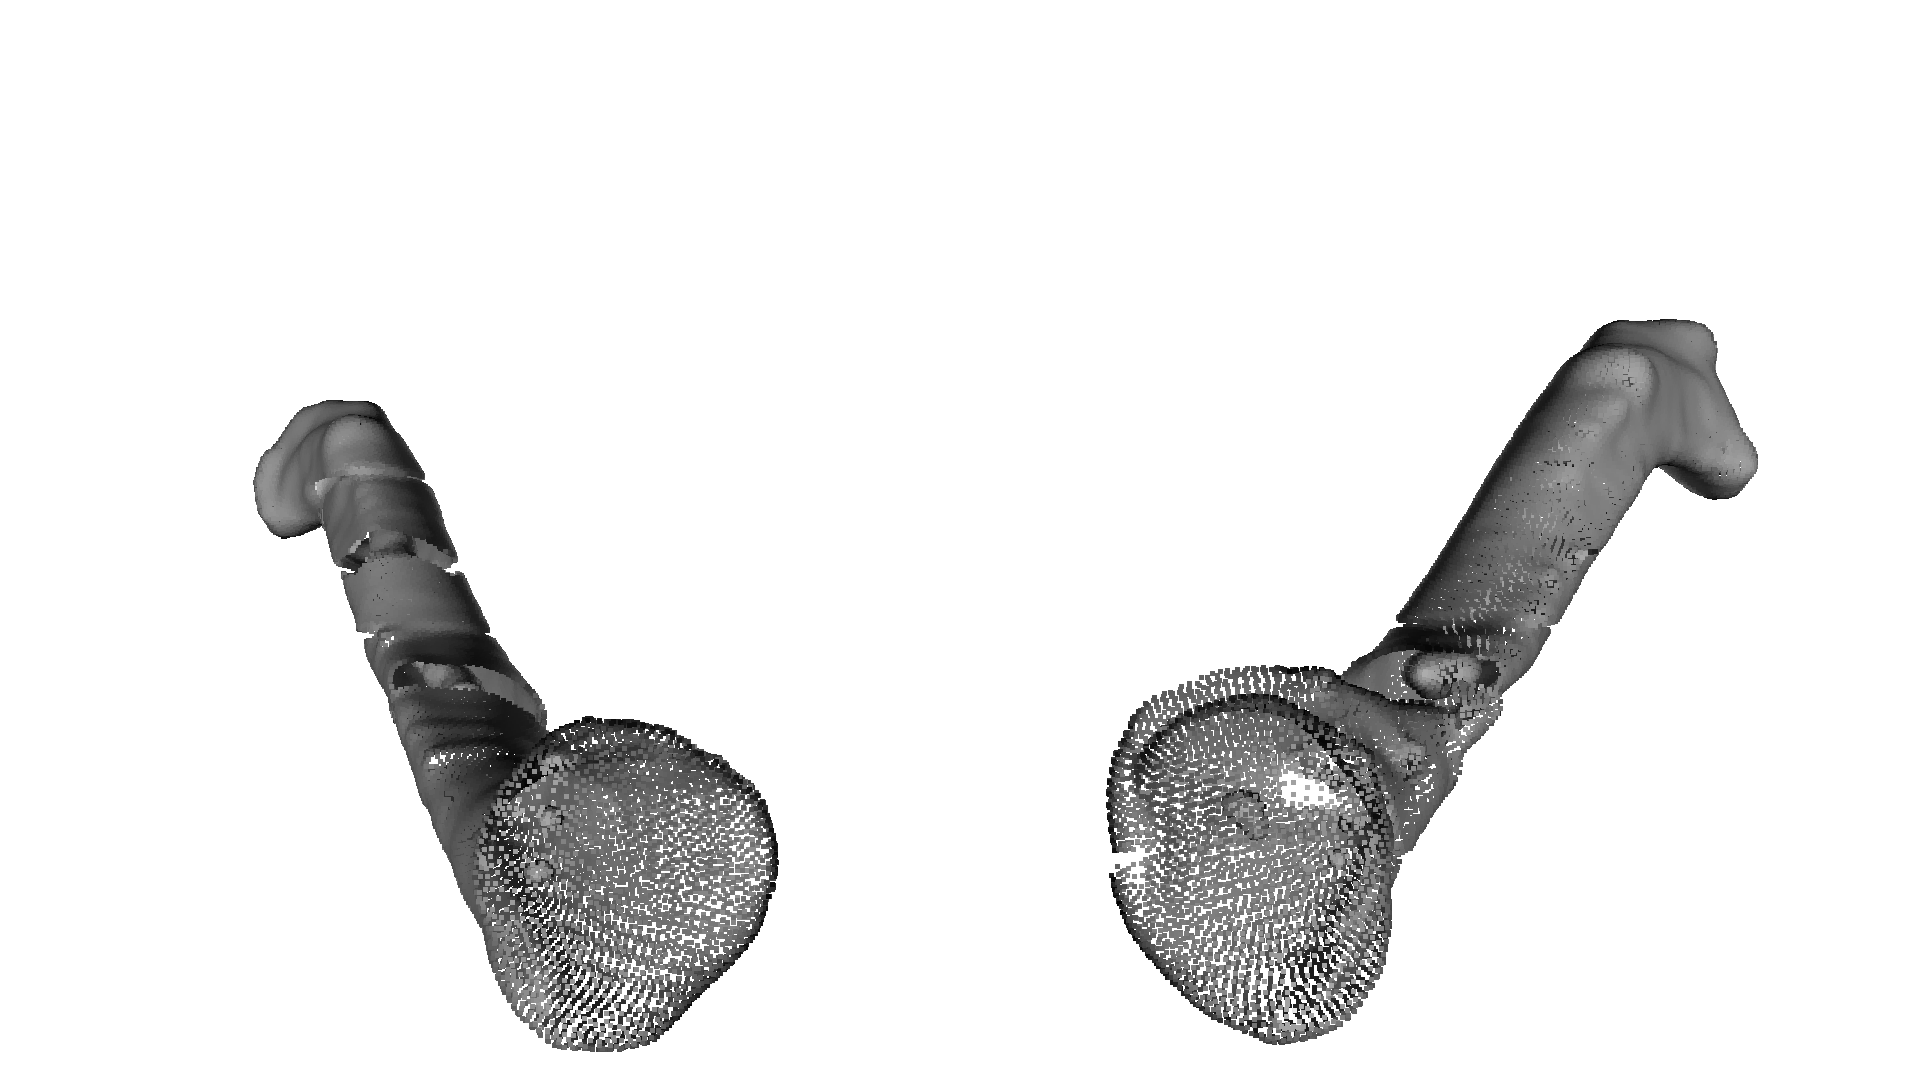
\includegraphics[width=.95\textwidth]{imagenes/chapter2/clavicula/clavicula_4.png}
    \caption{}
  \end{subfigure}
  \begin{subfigure}[b]{.5\textwidth}
    \centering
    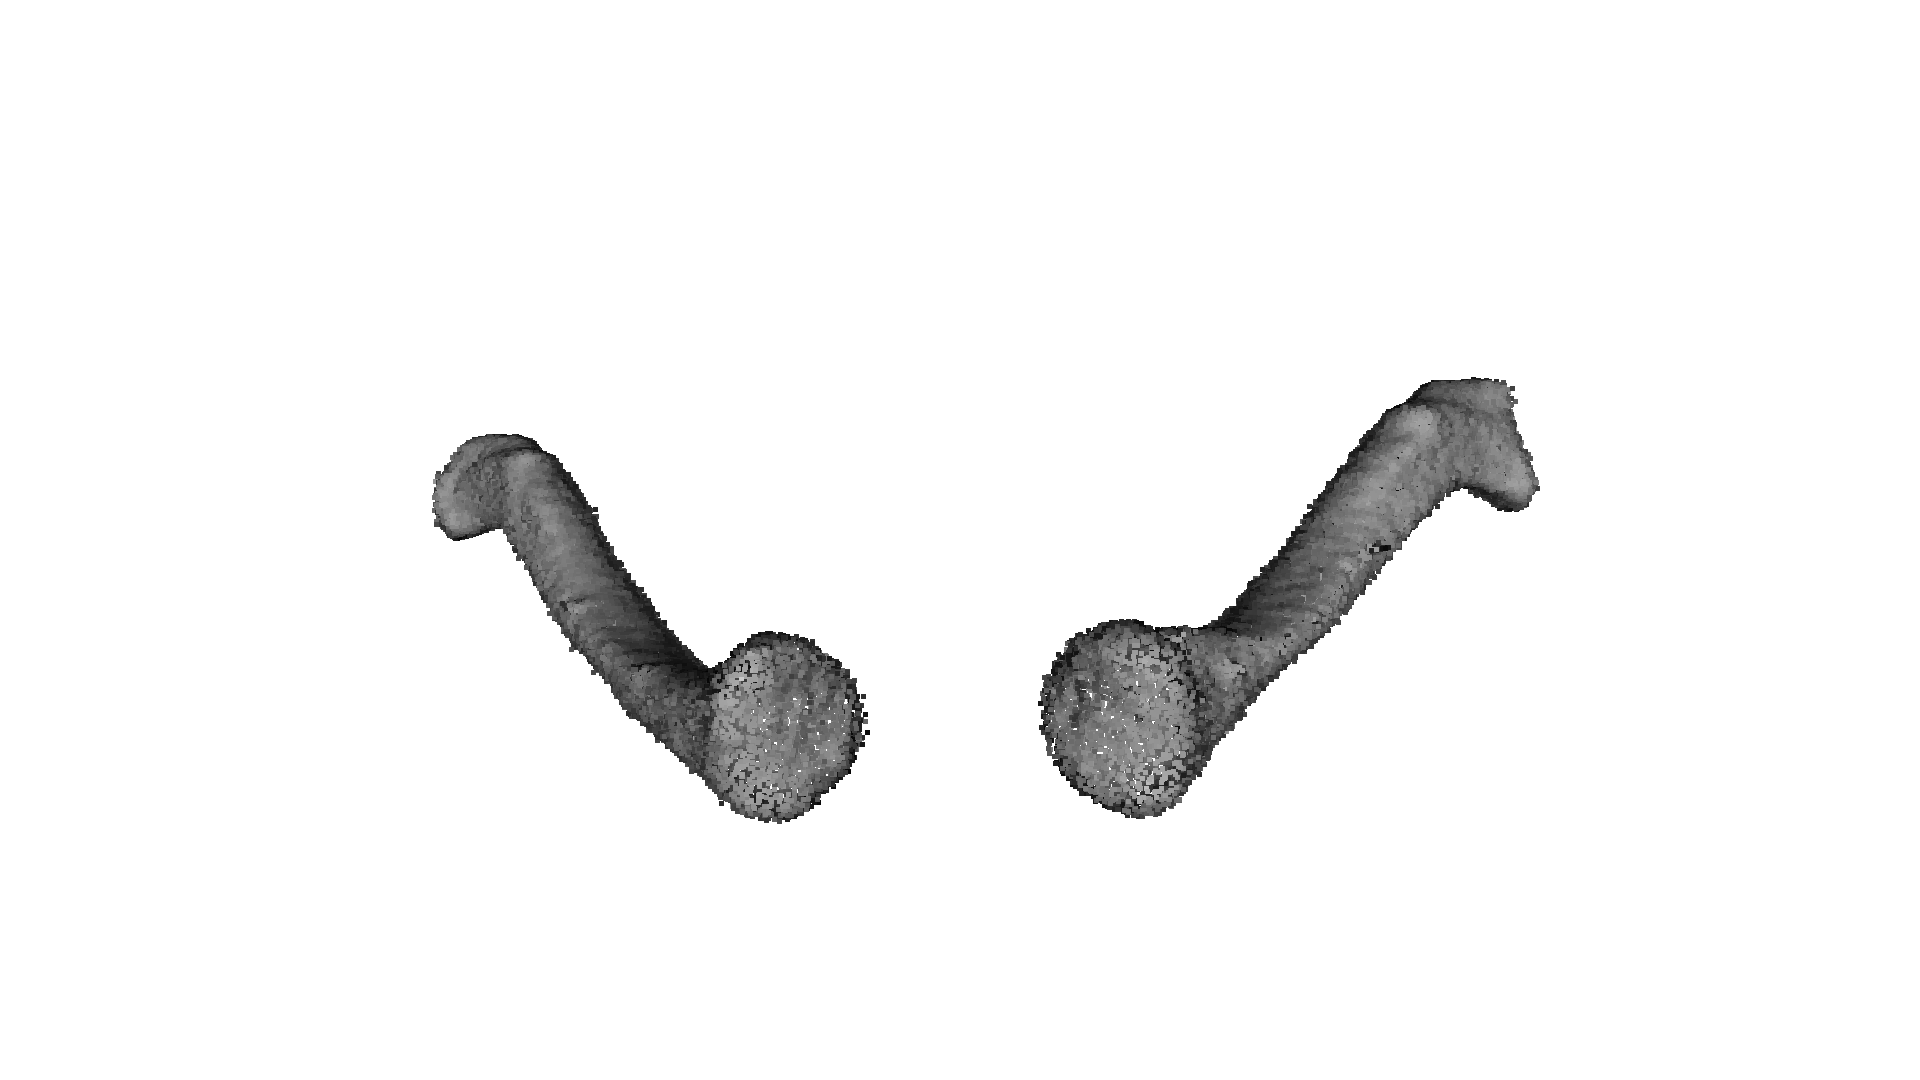
\includegraphics[width=.95\textwidth]{imagenes/chapter2/clavicula/clavicula_5.png}
    \caption{}
  \end{subfigure}
  \caption[Ejemplo de distorsiones generadas sobre clavículas.]{Ejemplo de distorsiones generadas sobre clavículas.
    Tenemos la imagen original (a) y luego su versión tras compresión \emph{octree} (b), 
    tras reducción de puntos por \emph{random downsampling} (c), tras simulación 
    de movimiento local (d) y rotación local (e), y, por último, ruido gaussiano (f).
  }
  \label{fig:DistorsionesGeneradas}
\end{figure}

En total tendremos: compresión \emph{octree}, submuestreo uniforme, movimiento local, rotación local 
y ruido gaussiano. Cada uno de estas distorsiones son 
aplicadas en 7 niveles crecientes de intensidad.
Las resoluciones de compresión \emph{octree} van de 0.4 a 1.0 en intervalos de 0.1.
El submuestreo aleatorio realiza una reducción del 10\% al 70\% de los puntos.
Tanto el movimiento como la rotación local se aplican de 1 a 7 veces.
Por último, el ruido gaussiano va de 0.15\%, 0.20\%, 0.25\%, 0.30\%, 0.35\%, 0.4\% y 0.5\% del \emph{bounding box}. 
Como resultado, tenemos un total de 385 ejemplos (véase Apéndice \ref{sec:DatosSinteticos}). 

\section{Métodos}
Como se pudo observar en la Sección \ref{sec:EstadoDelArte}, actualmente hay una 
tendencia, justificada, a los métodos de DL frente a ML. Sin embargo, se experimentará con 
ambos. No obstante, se tuvo 
que descartar o adaptar todos los métodos que tuvieran en cuenta información de textura, 
cosa que no existe en los volúmenes médicos habituales. También se descartaron 
modelos que utilizan información perceptual de regiones locales, ya que necesitamos 
dicha información respecto de la imagen en su totalidad. 
Ambas características son dificultades añadidas a la hora 
de resolver el problema. La primera restringe el problema 
a la estimación de calidad de las estructuras en la imagen, eliminando la 
percepción de calidad por contraste y saturación. La segunda incrementa 
la complejidad computacional. 

\subsection{Modelo NR 3D-QA}
\label{sec:NR3DQA}
Antes de probar directamente con modelos de DL, se experimentó con un método de 
ML basado en la extracción de características de escena y entrenamiento de un 
modelo de vectores soporte para la regresión. Para ello necesitamos definir 
que tipo de características queremos extraer. 

Zhang et al~\cite{NR3DQA} proponen utilizar características geométricas y de 
color. Para la primera, extraen la curvatura \eqref{eq:Curvatura}, 
anisotropía \eqref{eq:Anisotropia}, linealidad \eqref{eq:Linealidad}, 
planaridad \eqref{eq:Planaridad} y esfericidad \eqref{eq:Esfericidad} de los puntos. 
Estas características se pueden extraer del vecindario 
de un punto por medio de la matriz de covarianza y los valores singulares. 
Las fórmulas que las definen son: 
\begin{equation}
  Cur(p_i) = \frac{\lambda_3}{\lambda_1 + \lambda_2 + \lambda_3}
  \label{eq:Curvatura}
\end{equation}
\begin{equation}
  Ani(p_i) = \frac{\lambda_1 - \lambda_3}{\lambda_1}
  \label{eq:Anisotropia}
\end{equation}
\begin{equation}
  Lin(p_i) = \frac{\lambda_1 - \lambda_2}{\lambda_1}
  \label{eq:Linealidad}
\end{equation}
\begin{equation}
  Pla(p_i) = \frac{\lambda_2 - \lambda_3}{\lambda_1}
  \label{eq:Planaridad}
\end{equation}
\begin{equation}
  Sph(p_i) = \frac{\lambda_3}{\lambda_1}
  \label{eq:Esfericidad}
\end{equation}
Donde $\lambda_1$, $\lambda_2$ y $\lambda_3$ se refieren a los correspondientes 
valores singulares. Para la extracción de las características de color, primeramente 
convierten el espacio de color RGB en el espacio LAB mediante los siguientes 
pasos de transformación: 
\begin{equation}
  \begin{bmatrix} 
    X \\ Y \\ Z 
  \end{bmatrix}  = 
  \begin{bmatrix}
    2.7688 & 1.7517 & 1.1301 \\ 
    1.0000 & 4.5906 & 0.0601 \\ 
    0 & 0.0565 & 5.5942 
  \end{bmatrix} = 
  \begin{bmatrix}
    R \\ G \\ B 
  \end{bmatrix} 
  \label{eq:ScaleXYZ}
\end{equation}
\begin{equation}
\begin{cases}
  L &= 116f\left(\frac{Y}{Y_n}\right) - 16 \\ 
  A &= 500\left( f\left(\frac{X}{X_n}\right) - f\left(\frac{Y}{Y_n}\right) \right) \\ 
  B &= 200\left( f\left(\frac{Y}{Y_n}\right) - f\left(\frac{Z}{Z_n}\right)\right) 
\end{cases}
  \label{eq:LABTransform}
\end{equation}
Donde R, G y B son los correspondientes canales RGB de color. La función que 
determina la transformación final viene descrita por \eqref{eq:LABfun}: 
\begin{equation}
  f(t) = \begin{cases} \sqrt[3]{t} & \textrm{sí}\; t > \sigma^3 \\ 
    \frac{t}{3\sigma^2} + \frac{4}{29},& \textrm{en cualquier otro caso.}
         \end{cases}  
  \label{eq:LABfun}
\end{equation}
Donde $\sigma = \frac{6}{29}$.
Sin embargo, en el caso de las imágenes médicas estas características deben 
ser descartadas, dado que el color existente al visualizar las nubes de puntos 
médicas no son más que un valor sintético añadido previamente que permite 
una visualización más agradable de las mismas. 
Finalmente, estiman la entropía de cada una de las características 
ya que argumentan que existe una alta correlación entre la 
entropía y la distorsión por cuantización. 
Además, a las características geométricas se les calcula 
la distancia a las distribuciones gaussiana y gamma tras observarse 
que la distribución de estas se veía afectada por la intensidad 
de las distorsiones. 

Para cada tipo de característica, se utiliza el valor medio y la desviación típica 
obtenida para cada punto de la nube de punto. Por último, sobre estas medidas, 
para el conjunto de datos de entrenamiento se normaliza con \eqref{eq:MeanNorm}.
Donde F es la característica extraída y C una pequeña constante para la 
estabilidad numérica. El conjunto de test se normaliza utilizando las medias y 
desviaciones de los datos de entrenamiento.
\begin{equation} 
  \hat F = \frac{F-mean(F)}{std(F) + C}
  \label{eq:MeanNorm}
\end{equation}


\subsection{Modelo VQA-PC}
Zhang et al~\cite{VQA-PC} propusieron un modelo de estimación de calidad de nubes 
de puntos utilizando proyecciones 2D de diferentes perspectivas. 
Observaron que los métodos que trabajan directamente sobre la nube de puntos tienen
una elevada dificultad computacional, sin suponer una mejora excesiva, y que 
deben todavía madurar en el campo dado la alta complejidad de las nubes de puntos.
Por ello proponen utilizar proyección multi-vista. No obstante, argumentaron que 
los métodos anteriores de proyección se basan en la hipótesis de que los humanos 
percibimos la calidad de modelos 3D desde una perspectiva estática, cosa que no 
es cierta en la práctica dado que los objetos 3D permiten operaciones geométricas 
de rotación y escalado.
Y por ello, proponen unificar la percepción estática con la dinámica tratando 
a las proyecciones como vídeos.

De esta forma, se puede extraer características espaciales y temporales, como 
discutido en la Sección \ref{sec:VideoCNN}, utilizando redes convolucionales 
adaptadas a vídeos, de la familia \emph{SlowFast}~\cite{SlowFastNetworks}.
Siguiendo la motivación de que las deformaciones geométricas no deseadas se presentan 
de forma abrupta según la perspectiva (véase Figura \ref{fig:ViewPoint}), y que 
incluso se pueden observar incoherencias entre perspectivas adyacentes
utilizaron 4 ejes de rotación: vertical, horizontal, diagonal derecha 
y diagonal izquierda. Para cada eje se genera un total de 30 \emph{frames}, 
en total habrá 120 (véase Figura \ref{fig:VQARotation}). El ángulo de rotación es de 12 grados para todos los casos. 
Terminando la rotación de un eje en la misma posición inicial. 
A continuación se extraen características temporales del vídeo, que es posible 
generar a partir de cada \emph{frame} de los distintos ejes de rotación encadenados
secuencialmente de forma ordenada, y se elige 1 \emph{frame} de cada 
eje de rotación para representar la información espacial. Por último, 
tenemos que aprender una función de interacción entre los dos vectores característicos 
extraídos. Proponen concatenar los vectores y aprender una función por 
medio de una capa totalmente conectada utilizando el MSE.

\begin{figure}
  \begin{center}
    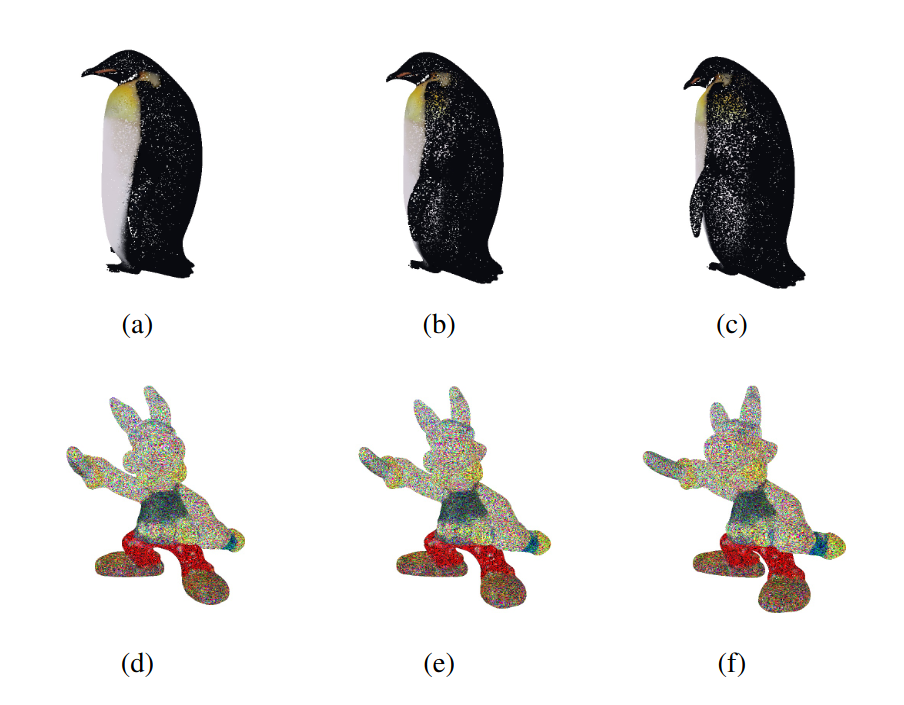
\includegraphics[width=0.75\textwidth]{imagenes/chapter4/ViewPoint}
  \end{center}
  \caption[Ejemplo de distorsiones que se presentan según la perspectiva]{
  Ejemplo de distorsiones que se presentan según la perspectiva.
Vemos que al girar el pingüino se empieza a observar un bajo número de puntos en su 
lateral izquierdo, permitiendo verse a través de él. De forma similar, 
en la imagen de abajo se ve cierta deformación de la cabeza.}
  \label{fig:ViewPoint}
\end{figure}

\begin{figure}
  \begin{center}
    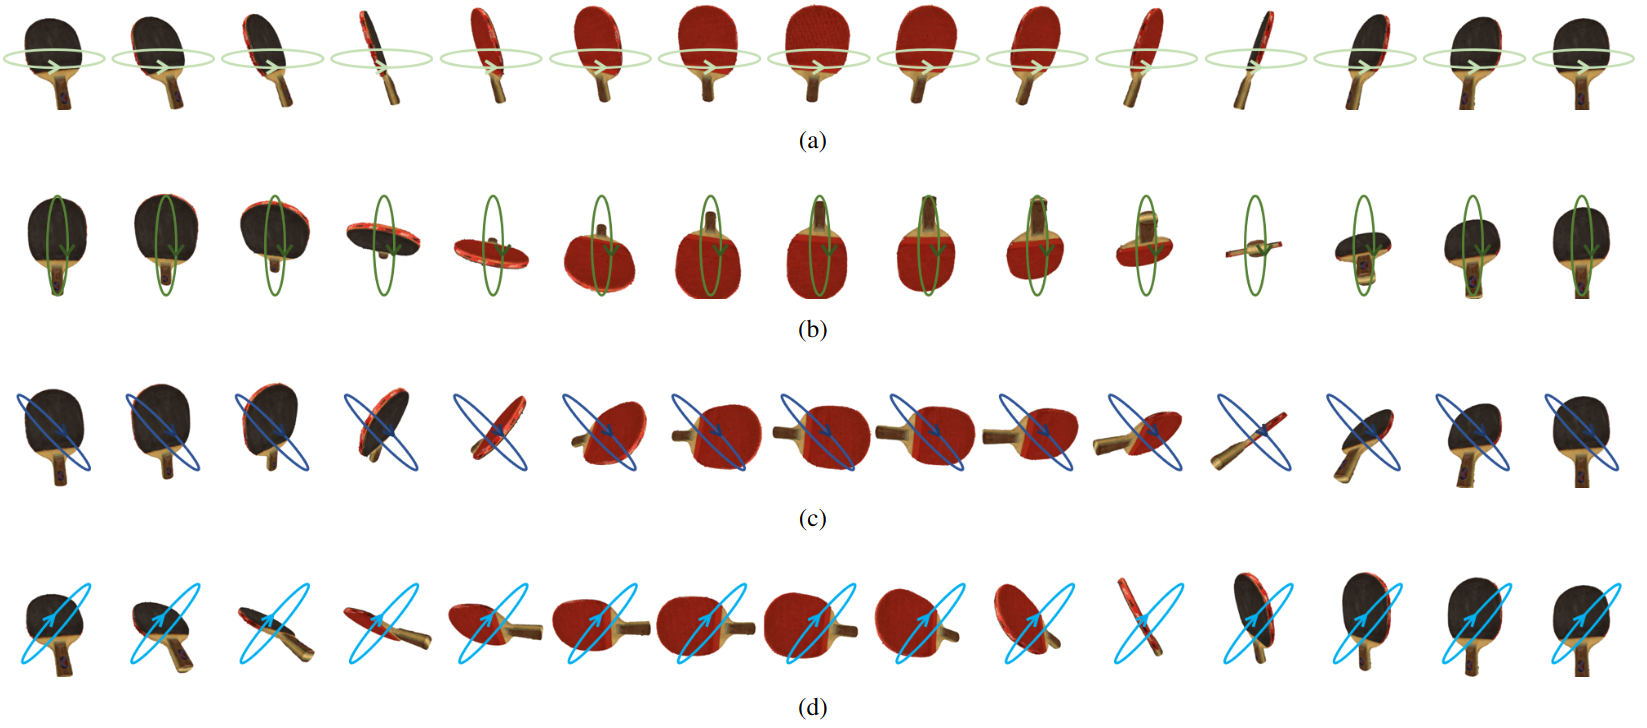
\includegraphics[width=.95\textwidth]{imagenes/chapter4/VQARotation}
  \end{center}
  \caption[Ejemplo de las rotaciones que utiliza el modelo VQA-PC.]
  {Ejemplo de las rotaciones que utiliza el modelo VQA-PC.
  Se observa que el final de cualquier eje de rotación es la posición inicial, 
permitiendo así unir suavemente una secuencia de imágenes encadenada de los ejes 
que genere un vídeo de rotación utilizado luego para la estimación.}
  \label{fig:VQARotation}
\end{figure}

Para realizar la secuencia de vídeo, necesitamos realizar correctamente 
el conjunto de rotaciones descritos por las siguientes ecuaciones: 
\begin{equation}
  \theta_A = 
\begin{cases}
\begin{aligned}
   X_\alpha^2 + Y_\alpha^2 & = R^2 \\ 
    Z_\alpha & = 0 
\end{aligned}
\end{cases}
\label{eq:RotationA}
\end{equation}

\begin{equation}
  \theta_B = 
\begin{cases}
\begin{aligned}
   Y_\alpha^2 + Z_\alpha^2 & = R^2 \\ 
    X_\alpha & = 0 
\end{aligned}
\end{cases}
\label{eq:RotationB}
\end{equation}

\begin{equation}
  \theta_C = 
\begin{cases}
\begin{aligned}
   X_\alpha^2 + Y_\alpha^2 + Z_\alpha^2 & = R^2 \\ 
    X_\alpha + Z_\alpha & = 0 
\end{aligned}
\end{cases}
\label{eq:RotationC}
\end{equation}

\begin{equation}
  \theta_D = 
\begin{cases}
\begin{aligned}
   X_\alpha^2 + Y_\alpha^2 + Z_\alpha^2 & = R^2 \\ 
    X_\alpha - Z_\alpha & = 0 
\end{aligned}
\end{cases}
\label{eq:RotationD}
\end{equation}

Y para llevar a cabo la rotación debemos calcular el punto medio de la nube 
de puntos por medio de la siguiente Ecuación \eqref{eq:PuntoMedio}:
\begin{equation}
  O_\sigma = \frac{1}{N}\sum_{n=1}^N \sigma_n
  \label{eq:PuntoMedio}
\end{equation}
Donde el $O_\sigma$ representa la coordenada (X,Y,Z) del centro medio de la 
nube de punto, y $\sigma_n$ representa la coordenada del punto $n$-ésimo punto. 
Utilizando ese centro, aplicamos las ecuaciones \eqref{eq:RotationA} a \eqref{eq:RotationD}.

Para extraer las características espaciales empleamos un modelo pre-entrenado, 
en concreto se investigaron variaciones de arquitecturas ResNet~\cite{ResNet}. Una 
familia de redes residuales, que en su momento resolvieron el problema 
del estancamiento en el entrenamiento de redes neuronales profundas debido 
a la degradación del gradiente. El único modelo al que optimizaremos sus pesos es 
ResNet, el modelo de extracción temporal solo es un paso previo.

\begin{figure}[H]
  \begin{center}
    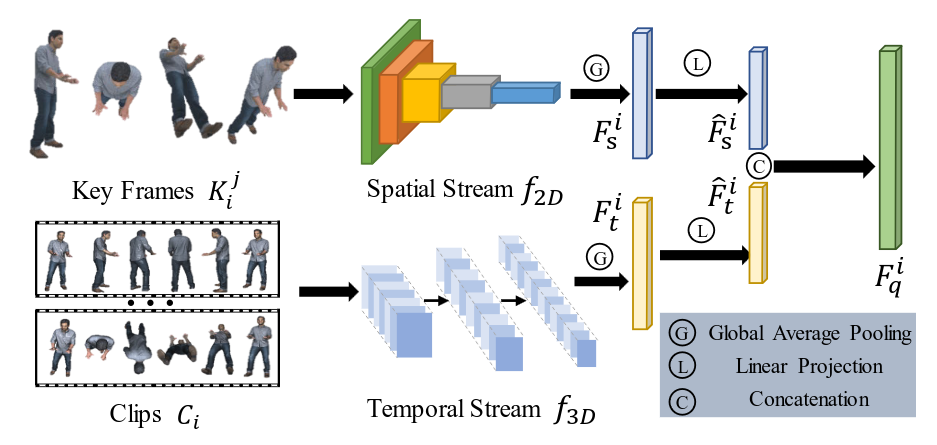
\includegraphics[width=0.60\textwidth]{imagenes/chapter4/PipelineCompleto}
  \end{center}
  \caption{Ejemplo detallado de las etapas del método de VQA-PC.}
  \label{fig:VQAPipeline}
\end{figure}

\section{Evaluación}
\subsection{Etiquetado}
Al tener que generar un conjunto de datos médicos por medio de la simulación 
de distorsiones a distintos niveles de intensidad, es también necesario una manera 
de etiquetar cada ejemplo generado con el valor de calidad esperado. 
Para la generación de dicha etiqueta, se optó seguir el camino propuesto por~\cite{ResSCNN}. 
En opción a generar un entorno controlado con los estándares ITU-R~\cite{ITU-R.2012, ITU-R.2021}, 
organizar al menos 16 personas, y que cada uno evalúe durante 30 segundos el nivel 
de calidad de cada nube de punto en una escala 1-5, hemos hecho uso del gran 
avance de las métricas con referencia que poseen un alto nivel de correlación con 
la percepción de calidad del observador final. 
Para ello, se hace un desglose de rendimiento de cada métrica para cada tipo 
de distorsión, como se observa en la Tabla \ref{tab:MetricsPerDistortion}. El 
rendimiento es medido con el coeficiente de correlación de rangos de Spearman.
Las métricas comparadas son p2p0~\cite{PointToPoint} y p2pl~\cite{PointToPlane}, 
con distancia manhattan (M) y hausdorff (H), PCQM~\cite{PCQM}, GraphSIM~\cite{GraphSIM} y 
MPED~\cite{MPED}.

\begin{table}[htp]
    \scriptsize
    \hspace{-.7cm}
    \begin{tabular}{|c|c|c|c|c|c|c|c|}
    \hline
        \rowcolor[HTML]{FFC702} 
        \textbf{Distortion} & \textbf{M-p2po} & \textbf{M-p2pl} & \textbf{H-p2po} & \textbf{H-p2pl} & \textbf{PCQM} & \textbf{GraphSIM} & \textbf{MPED} \\ \hline
        DownSample & \textbf{0.881} & 0.626 & 0.841 & 0.811 & 0.524 & 0.842 & 0.857 \\ \hline
        GaussianShifting & 0.741 & 0.718 & 0.829 & \textbf{0.834} & 0.816 & 0.742 & 0.598 \\ \hline
        LocalOffset & \textbf{0.937} & 0.934 & 0.770 & 0.770 & 0.851 & 0.906 & 0.897 \\ \hline
        LocalRotation & 0.819 & 0.712 & \textbf{0.831} & 0.734 & 0.657 & 0.723 & 0.742 \\ \hline
        Octree & 0.779 & 0.788 & \textbf{0.819} & 0.752 & 0.676 & 0.757 & 0.710 \\ \hline
    \end{tabular}
    \caption[Tabla de métricas para generación de etiquetas.]{
      Tabla de métricas para generación de etiquetas extraídas de~\cite{ResSCNN}.
  }
    \label{tab:MetricsPerDistortion}
\end{table}

En~\cite{ResSCNN} validaron sus muestras generadas con las métricas del estado del arte 
para el subproblema FR por medio de un análisis subjetivo con el estándar ITU-R, en
un entorno controlado, definido anteriormente, y obtuvieron una correlación del 
90\% entre las muestras 
etiquetadas subjetivamente y las que fueron etiquetadas objetivamente (véase Tabla \ref{tab:PseudoCorr}).
Con ello, se logra justificar la generación de las etiquetas como una sustitución 
de los métodos de evaluación subjetivos. 

\begin{table}[H]
  \centering 
  \scriptsize
  \begin{tabular}{|c|c|c|}
    \hline
    \rowcolor[HTML]{FFC702}
     & \textbf{Parte I} & \textbf{Parte II} \\
    \hline 
    SROCC & 0.902697 & 0.878517\\
    \hline
    PLCC & 0.910713 & 0.871917\\
    \hline
  \end{tabular}
  \caption[Correlación de métricas sintéticas.]{
  Correlación de métricas sintéticas extraídas de~\cite{ResSCNN}.
  Donde ``Parte I'' y ``Parte II' se refieren a dos conjuntos de datos etiquetados 
  manualmente. El primero se utiliza para la elección de las métricas y el segundo 
  para test.
}
  \label{tab:PseudoCorr}
\end{table}

\subsection{Métricas de similitud}
\label{sec:Metricas}
Las métricas más utilizadas en la resolución del problema de estimación de calidad 
de imágenes suelen ser: el coeficiente de correlación de rangos de Spearman (SROCC, 
por sus siglas en inglés), el coeficiente de correlación lineal de Pearson (PLCC), coeficiente de correlación de orden de rango de Kendall (KROCC)
y raíz del error cuadrático medio (RMSE)~\cite{VisualMedicalQualityBook}.

Las tres primeras al ser coeficientes de correlación toman valores en el intervalo 
[-1, 1]. Siendo el valor -1 una correlación negativa entre los datos, es decir,
ambos decrecen en el tiempo. Al contrario, cuando esta es +1, tenemos una relación 
positiva que implica un crecimiento en el tiempo. Sin embargo, cada una de ellas 
miden la correlación de forma distinta. 

PLCC es una métrica que mide la correlación lineal entre dos conjuntos de datos.
Evalúa si existe una relación lineal entre los valores de ambos conjuntos.
Si definimos $x$ e $y$ como los vectores que contienen las puntuaciones de 
calidad objetiva y subjetiva de $m$ imágenes, siendo $x_i$ e $y_i$ 
los elementos contenidos en la posición $i$, entonces podemos formular 
PLCC como la Ecuación \eqref{eq:PLCC}.

\begin{equation}
  PLCC(x,y) = \frac{\sum_{i=1}^m (x_i - \bar x)(y_i - \bar y)}{\sqrt{\sum_{i=1}^m (x_i - \bar x)^2}\sqrt{\sum_{i=1}^m (y_i - \bar y)^2}}
\label{eq:PLCC}
\end{equation}

Como mencionado en \cite{ResSCNN} o \cite{VQA-PC}, se sugiere una transformación 
no lineal para las puntuaciones objetivas antes de calcular el PLCC y el RMSE.
Para ello utilizaremos la función de regresión logística-5, con 5 parámetros a aprender,
como en la Ecuación \eqref{eq:LG5}. 

\begin{equation}
  Q = \beta_1 \left(\frac{1}{2} - \frac{1}{1+e^{\beta_2 (Q_s-\beta_3}} \right) + \beta_4 Q_s + \beta_5
  \label{eq:LG5}
\end{equation}
Donde $Q$ es el valor final normalizado, $Q_s$ es el valor predicho y $\beta_i$ se 
refiere a los parámetros a aprender.
La elección se debe al análisis comparativo entre esta, logística-4, con 4 parámetros, y la función de regresión cúbica-4
desarrollado en~\cite{ResSCNN}. Los resultados se pueden ver en la Tabla \ref{tab:CompareNonLineal}, 
y las fórmulas adicionales en el Apéndice \ref{ape:Formulas}.

\begin{table}[htp]
  \centering
  \scriptsize
  \begin{tabular}{|c|c|c|c|}
    \hline
    \rowcolor[HTML]{FFC702} 
    & \textbf{Logística-4} & \textbf{Logística-5} & \textbf{Cúbica-4} \\
    \hline 
    SROCC & 0.8572 & \textbf{0.9026} & 0.8957\\
    \hline
    PLCC & 0.8626 & \textbf{0.9107} & 0.9044 \\
    \hline 
  \end{tabular}
\caption[Comparativa entre funciones de normalización.]{Comparación de la correlación entre dos conjuntos de datos, la etiqueta y 
  la predicción, tras utilizar las diferentes técnicas de normalización no lineal. 
Vemos que hay una mayor correlación entre los datos si se normalizan con la 
función logística-5.}
  \label{tab:CompareNonLineal}
\end{table}
También podemos no depender de la escala de los datos, para ello tendríamos que 
utilizar SROCC.
Esta es una métrica que mide la correlación de clasificaciones o \emph{rankings} entre 
dos conjuntos de datos. Evalúa si el orden relativo de los elementos es similar 
en ambos conjuntos. Por ello, es también invariante a transformaciones monótonas 
en los datos. Se puede formular como la Ecuación \ref{eq:SROCC}.

\begin{equation}
  SROCC(x,y) = \frac{\sum_i (x_i - \bar x)(y_i - \bar y)}{\sqrt{\sum_i (x_i - \bar x)^2}\sqrt{\sum_i (y_i - \bar y)^2}}
\label{eq:SROCC}
\end{equation}

De hecho, la correlación de rangos de Spearman es equivalente a calcular 
la correlación de Pearson sobre los rangos de los valores de entrada.

\begin{equation}
SROCC(x,y) = PLCC(rank(x), rank(y))
\label{eq:SROCCasPLCC}
\end{equation}

KROCC es una métrica similar a SROCC, pero utiliza el coeficiente de correlación 
de rangos de Kendall. También evalúa la correlación entre clasificaciones o \emph{rankings},
pero se basa en la concordancia o discordancia de los pares de elementos en los 
conjuntos.

\begin{equation}
  KROCC(x,y) = \frac{C-D}{\frac{1}{2} m (m-1)}
\label{eq:KROCC}
\end{equation}

Donde $C$ alude a cuantos pares de datos, x e y, están bien correlacionadas, 
y $D$ es el número de pares discordantes.  

Por último, RMSE es una métrica que mide la diferencia entre los valores 
predichos y los valores reales en un conjunto de datos. 
Calcula la raíz cuadrada del promedio de los errores al cuadrado. 
Un valor de RMSE más bajo indica un mejor ajuste o precisión del modelo.

\begin{equation}
  RMSE(x,y) = \sqrt{\frac{1}{m}\sum_{i=1}^m (x_i - y_i)^2}
\label{eq:RMSE}
\end{equation}



